\part{Analysis}
In this section, we will attempt to give the reader insight into the rationale behind the decisions made in the course of the project, by reflecting on challenges and surprises uncovered by analysing the problem area. In other words, the section will try to explain \textit{why} the system has been designed as it has and why the process has been managed the way it has.

The section is structured by the various techniques and artefacts used in conducting the analysis. The primary topics covered in this section are:
\begin{itemize}
\item Business modelling
\item Requirements analysis
\item Data modelling
\item Architectural analysis
\end{itemize}
We begin the section by investigating and discussing the conceptual business model of the system.

\section{Business modelling}
The following will present a business model, which will demonstrate the main ideas behind the our conceptualized system, the advantages and the possible threats.

Throughout the extreme growth of the usage of the Internet, a similar growth has been seen for user-uploaded content, which have explode on sites like www.youtube.com and www.facebook.com. Especially media files, like video and picture, has surfaced all over these sites, mainly due to the fore coming of smartphones, with picture and video capturing capabilities. The content of these media files is often self-exposing, where people capture themselves or friends doing all kinds of different things and at different events. But other media file content is also extremely popular to upload, like news broadcasting, sport events, tutorials, movies etc. Our business concept will focus on tutorials.

Tutorials have been widely exposed on Internet, where people are using the Internet increasingly to find solutions on how to do things themselves. Because of this, we have decided to develop a system, where a user can download and upload homemade tutorials and get paid for providing these files for the system. The payments will be financed through advertisements on the tutorials or by user payment, when a user is buying a video tutorial. The users will also be able to search video tutorials by category, ratings on videos and tags.

\subsection{Target group}
The target group is expected to posses general IT knowledge and know how to use a computer at a basic level. The system will target users that want to learn how to do things at home and by themselves and users that wants to learn about a special topic. The system will focus on tutorials of a specific subject, technology, and subjects comprised in this. This also means, that the users will have to have some kind of interests which can be related to technology, since the system will only contain video tutorials of this sort.
We have chosen not to focus on the following groups: Children, people above the age of 60 and handicapped people.

\subsection{Threats}
When developing a system like this, there will always be either threats or weaknesses, or both, related to the system. In this case, the most obvious threat, is the the competition from other similar sites. Video tutorials is a big part of the Internet and therefore there already is a lot of websites and programs, that offers the same content to users. And on top of that, users will have to pay for videos without advertisements on this system, which similar sites and programs offers for free. Another threat is the fact that the video content for the users, will be user generated and for at start, this content will be very limited, until the system have been exposed and users starts to upload tutorials.

\subsection{Strengths}
This system has a lot of strengths associated with it and will have a great chance to greatly impact the target user group. One of the major strengths of the system, is that all tutorials will be gathered in one place. Often when searching for information on how to do stuff, its needed to look in several places and sites, and this is always time consuming and frustrating. For this system, all tutorials for all subjects for technology will be in one place and give the users easy access to many related tutorials. On top of this, if a user chooses to upload a video, that user will get a chance to earn money for every view and download of the tutorial. This will also encourage the users who wish to upload tutorials, to make the tutorial in a good quality and with a great content, since this will increase their chance of getting earning more money, which will benefit the system.

In the preceding text, have the system been explained and the major aspects outlined. The system will contain video tutorials regarding technology and every subject under this, which the users can either see with advertisements or buy without advertisements. The tutorials will be uploaded by users and these users will earn money for each time their tutorial is either viewed or bought.
The system have both strengths and threats, which have been discussed in the above. These will be taken into consideration when developing the final system and the threats.
(Needs a little bit more wrap up)

\section{Requirements Analysis}
Generally speaking, requirements can be divided into two categories; functional and non-functional. The functional requirements for the RentIt server are expressed by use-cases, that each encapsulate some functionality the system must posses in order to be a useful solution. The non-functional requirements are captured by the factor-tabel.
  These artefacts will serve as the basis for the discussion of the requirements in this section.
\subsection{Use Cases}
As mentioned, the use-cases capture the functional requirements of the system. The list of use cases was composed by examining the business model and identifying user goals associated with uploading, viewing and buying videos, creating user accounts and so on.

When writing use cases for the RentIt system, we noted that they could be grouped into three categories of usage:
\begin{itemize}
\item \textbf{User management}\\
Use cases concerning user profile creation, editing user profiles and authorizing users
\item \textbf{Video management}\\
Use cases concerning downloading, viewing and rating videos
\item \textbf{Transaction management}\\
Use cases concerning transactions between account balances and buying more RentIt credits.
\end{itemize}
In other words, the use cases reveal at least three major areas of responsibility within the required functionality of the system. These responsibilities imply a large scale organization of namespaces, by way of the GRASP principles.

In addition, the use cases provided some intuition about the control flow of some of the major operations of the system. Take for example user case no. 11, which describes paying for a video:\\

\textbf{A user wishes to pay for a video}
\begin{itemize}
	\item Precondition: The user has an active account with sufficient money deposited
	\item Postcondition: The user has the appropriate amount withdrawn from his 				account
	\item Postcondition: The user is granted access to the video
	\begin{enumerate}
		\item The user finds the video he wants to buy
		\item The user indicates that he wants to buy the video
		\item The user is granted access to the video
	\end{enumerate}
\end{itemize}

While short and simple, the pre- and postconditions as well as the steps involved in the use case, reveal a number responsibilities and changes in control flow to be considered. For example, the precondition indicates that each user has a balance associated with her account, to which deposits are made  in a separate use case (no. 9). Furthermore, the following responsibilities need to be delegated to appropriate branches of the system
\begin{itemize}
\item withdrawing money from the users account
\item granting users access to videos upon successful payment
\end{itemize}
This insight can be used as inspiration when designing the large scale organization of namespaces, and the control flow between these packages.

Moreover, the use cases proved an effective way of communicating ideas with the SMU group. By comparing our use cases with their use case model, it was possible to reconcile the two groups expectations to the semantic meaning of the different operations of the system. Take for example use case no. 4, dealing with purchasing videos:\\

\textbf{A user wants to see a video and downloads it to his computer}
\begin{itemize}
\item Precondition: User is logged in
\item Precondition: User has enough credits to pay the video
\item Postcondition: The video is saved on the users computer
\item Postcondition: The appropriate amount is subtracted from the users account
\begin{enumerate}
\item Available videos are presented to the user
\item The user selects the video he wants to see
\item The user is presented with options to rent and buy
\item The user selects buy
\item The user specifies where the file should be saved
\item The download begins
\end{enumerate}
\end{itemize}

This use case was utilized as the basis of a discussion between our own and the SMU group, about the semantic meaning of the term "buy", by the end of which it was decided that downloading a video constituted a buy, whereas renting would involve streaming the video, which is also expressed in the use case.

\subsection{Factor Table}
As opposed to the functional requirements, the non-functional requirements are not expressed by some functionality the system must offer, but rather some behaviour or quality the system must posses. These are captured by a factor table, as described in \textbf{Larman}. The list of factors the factor table consists of, was devised by using the FURPS+ mnemonic, and brainstorming on predictable requirements based on the business model. This facilitated a fruitful discussion on topics such as security, reliability and performance requirements of the system. The factor table can be found below:
\begin{center}
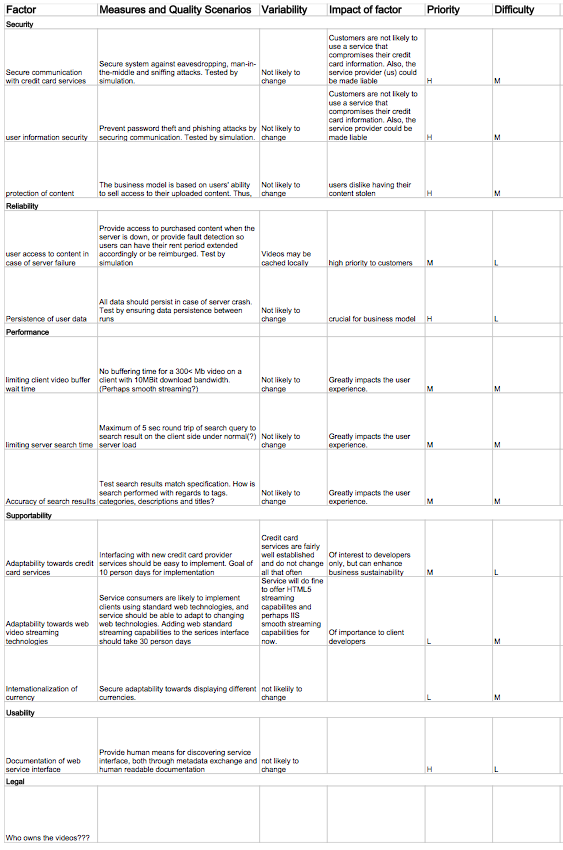
\includegraphics[scale=1.3]{FactorTable.png}
\end{center}
The factors are mainly defined by the business model, in that making changes to the business model, would change the non functional requirements of the system.  For example, the decision to include user generated content greatly impacts factors such as protection of video content in the system, as this in some sense the property of the user who uploaded it.

Some of the usefulness of the factor table is its recording of quality scenarios, because it encouraged the group to reflect on the quantifying the requirement, as to make it testable. Realistically, it would not be possible to satisfactory implement and test all of the factors, but for the sake of exercise, the factor table was composed as if it was meant to be used in  real world situation. As a consequence of the limited timeframe of the project, we decided to limit the factors that we would \textit{actually} emphasize to:
\begin{itemize}
\item accuracy of search results
\item documentation of web service interface
\item persistence of user data
\end{itemize}

These factors were consensually understood as the most crucial and/or interesting requirements to pursue.

\section{Data Modelling}
Another major part of our problem analysis was devising a model of the data, partly in order to construct and refine a database design for persisting the necessary data, and in part to serve for inspiration for C\# classes.
This modelling was done using two artefacts, a domain model to serve as a visual dictionary for objects and concepts in the problem domain, and an ER-diagram as an aid for reflecting on a useful database design. These two artefacts serve the basis for discussions in this section.
\subsection{Domain Model}
Something about the domain model
%The domain model was used to facilitate and document the results of a %discussion of the problem domain. By modelling the objects and concepts in the %problem domain, the project group came upon a number of questions, such as:
%\begin{itemize}
%\item 	
%\end{itemize}
\begin{center}
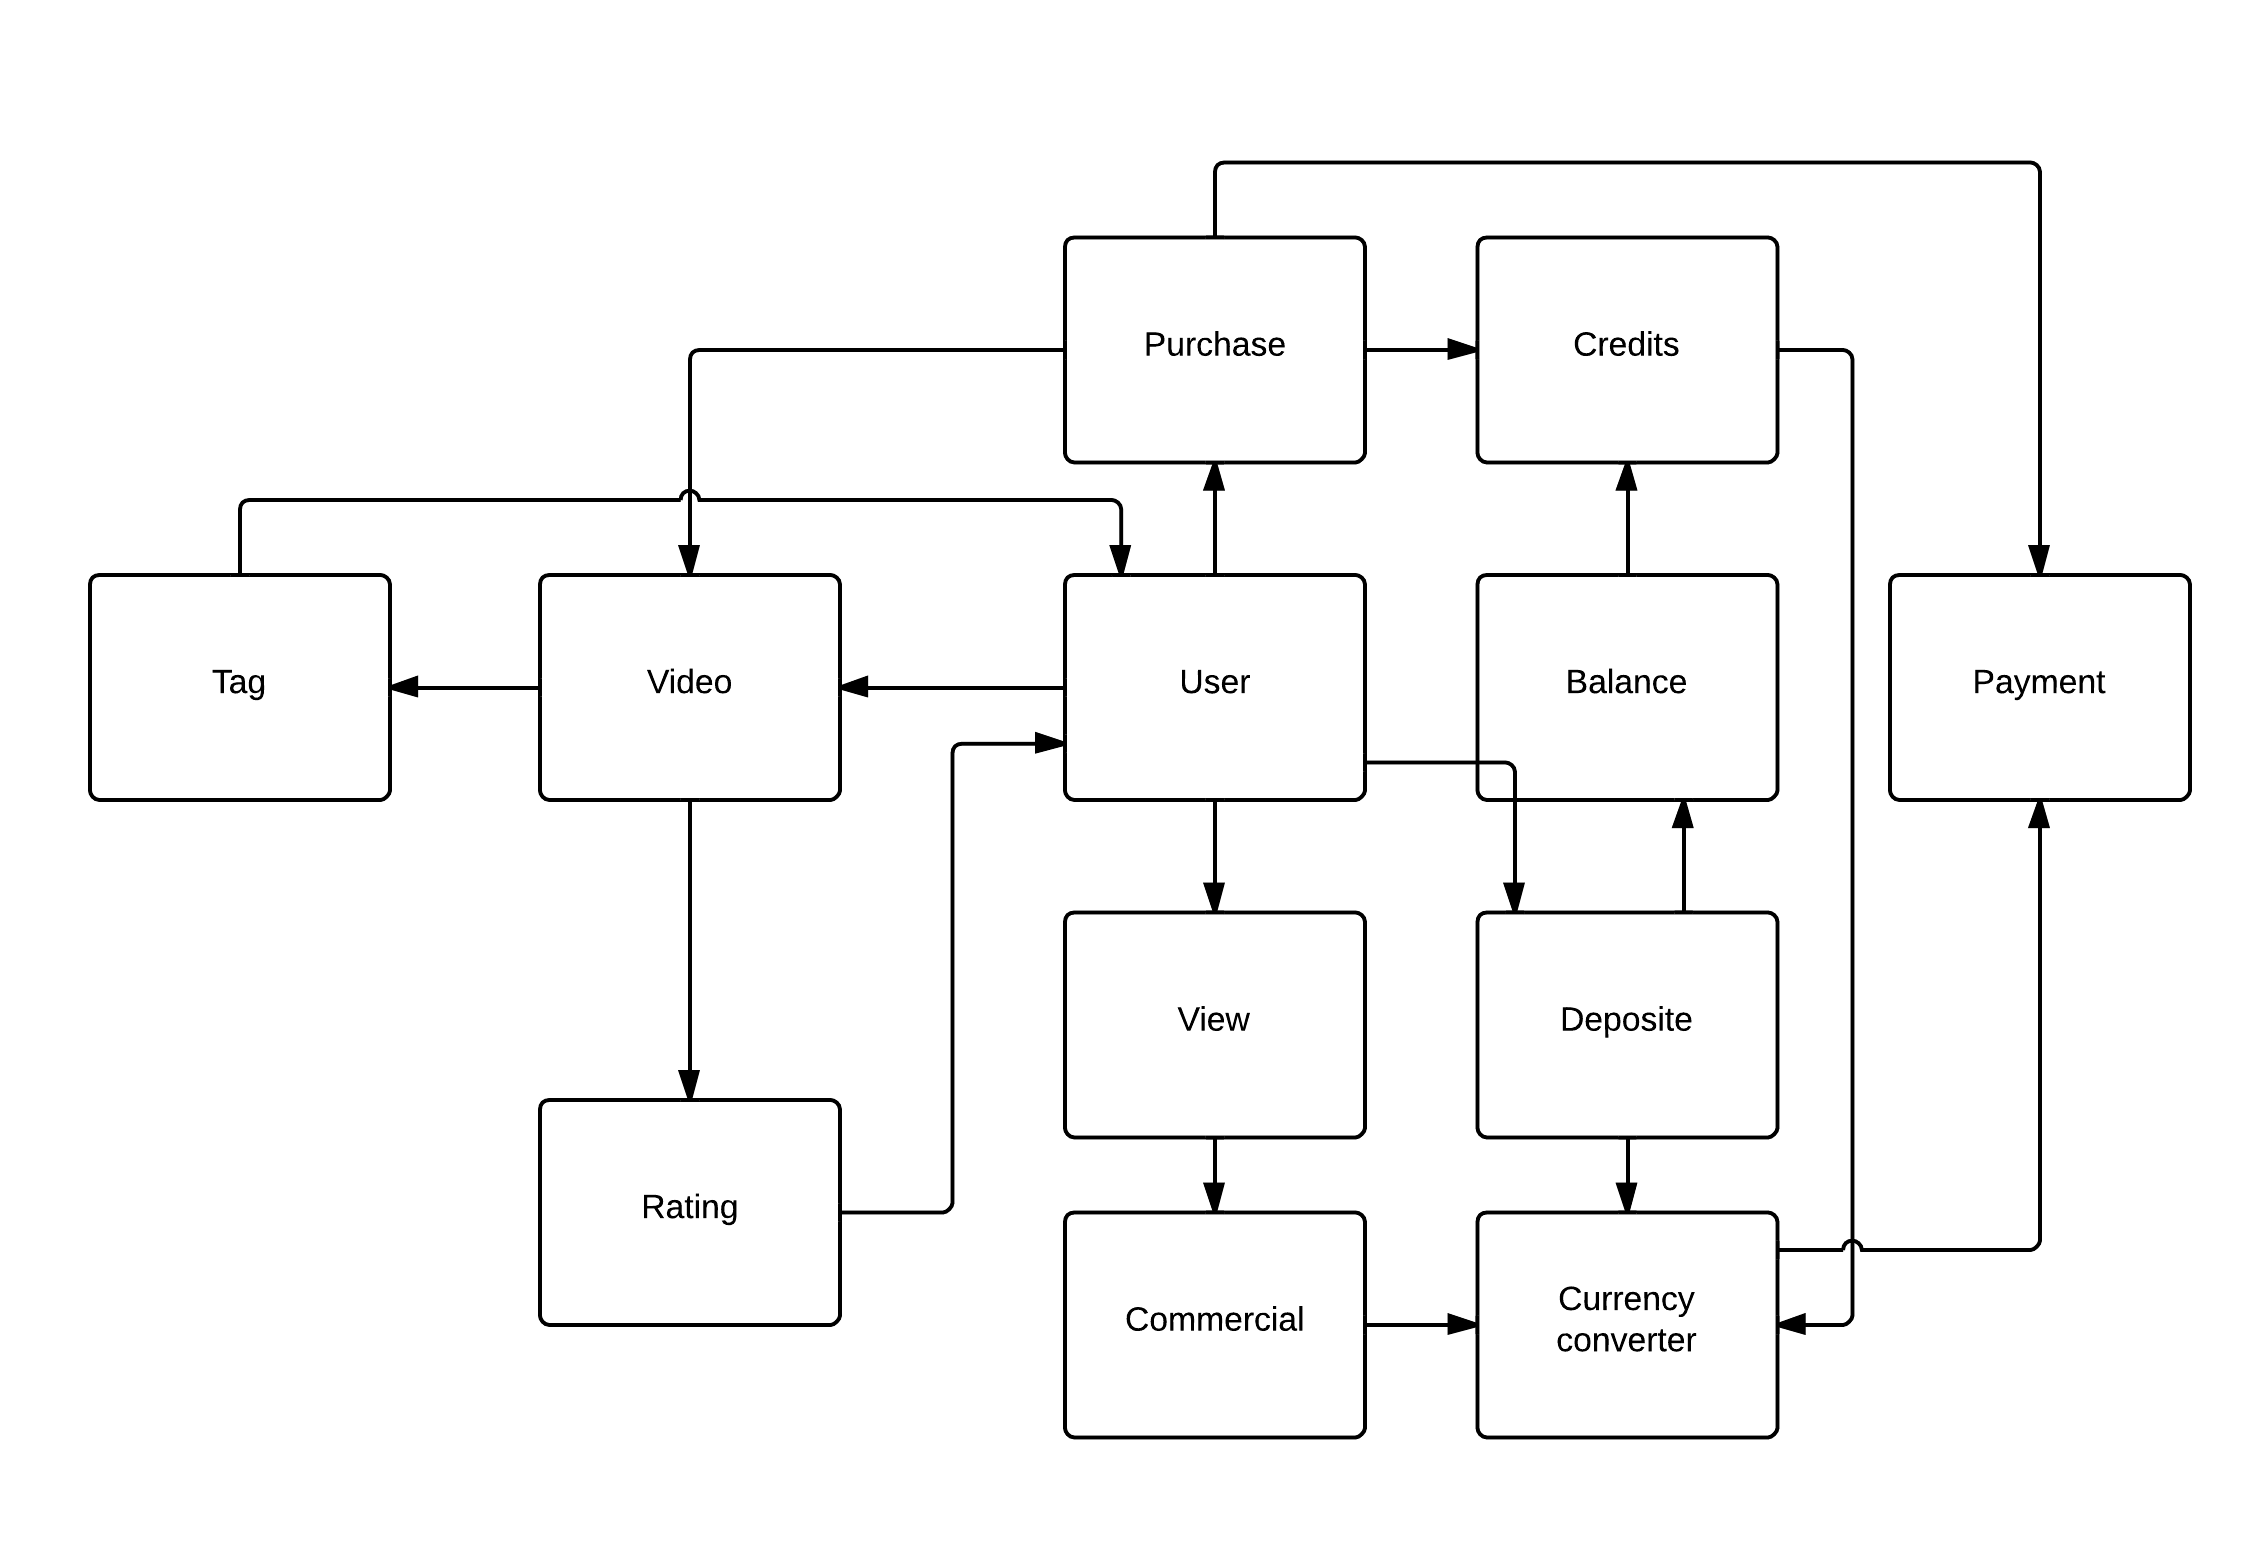
\includegraphics[scale=0.15]{DomainModel.png}
\end{center}

\subsection{ER-Diagram}
The ER diagram on the following page reflects our considerations on which data should be captured and persisted by the system. The video and user entities constitute the bare minimum of required data to implement the core functionality of video streaming and user management, and the remaining entities capture the data needed to record either deposits and payments, or the data needed to perform statistical analysis for e.g making recommendations to individual users.
\begin{center}
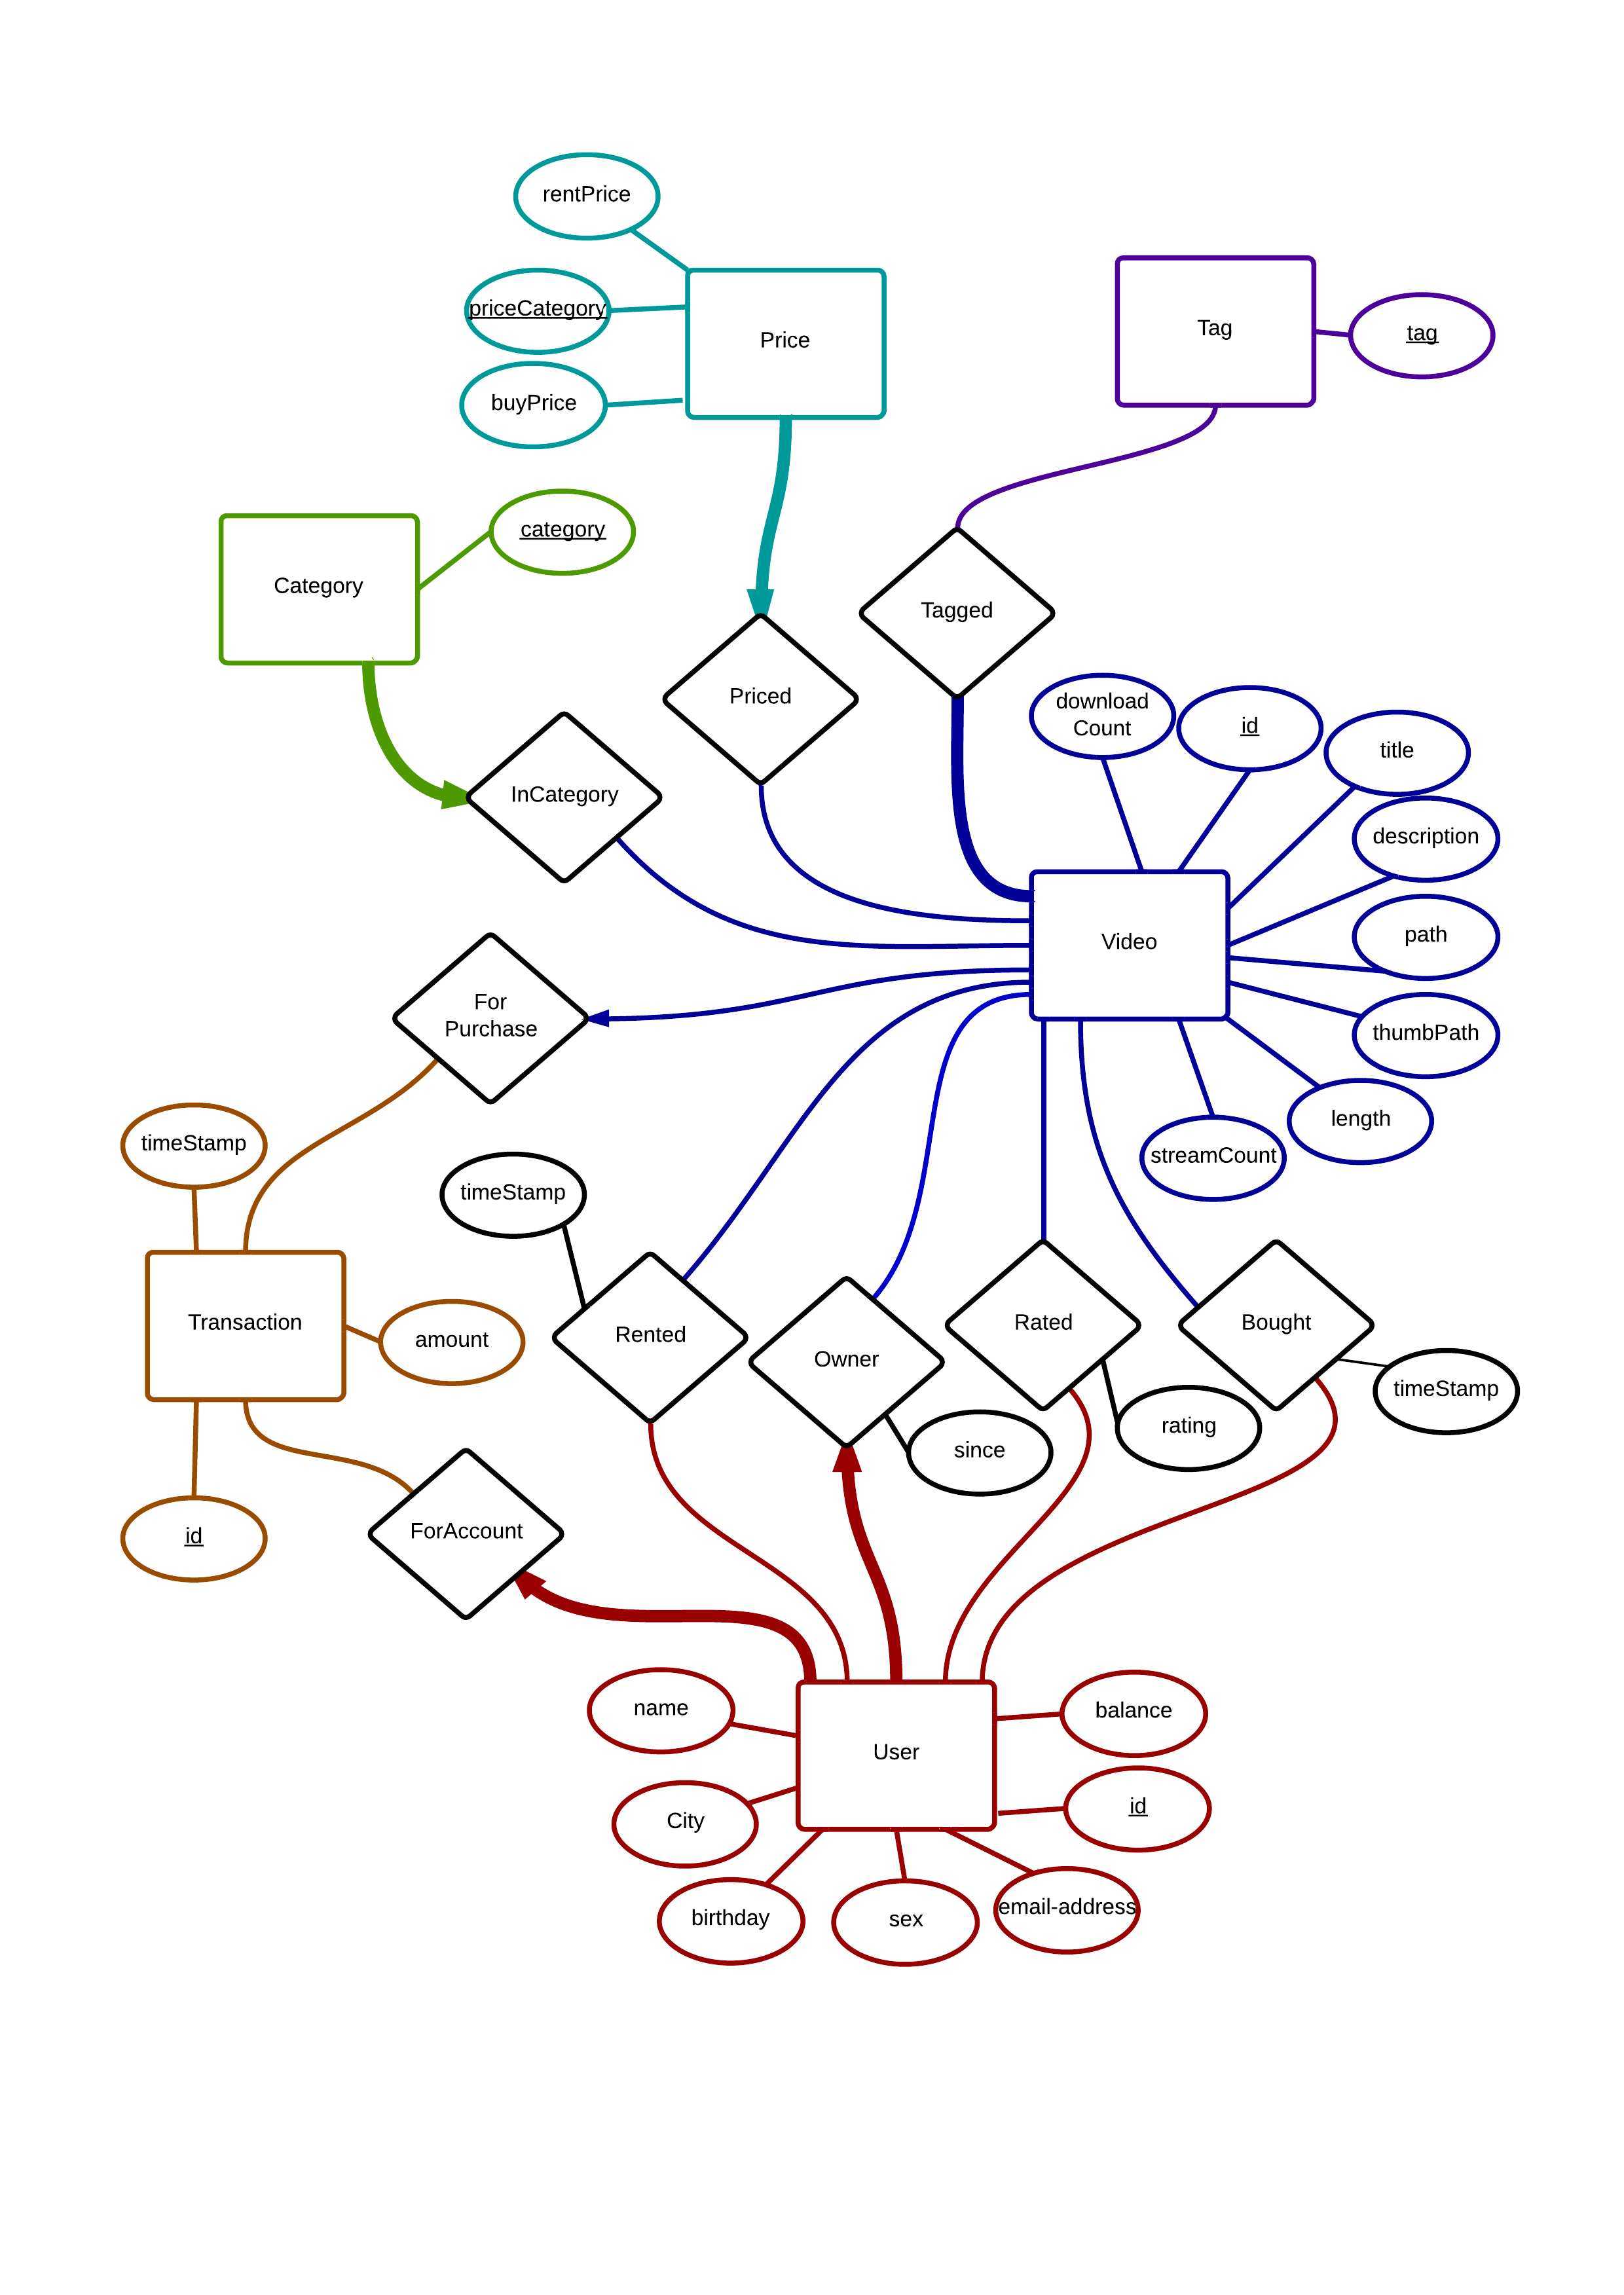
\includegraphics[scale=0.15]{ERDiagram.png}
\end{center}
The transaction, rented and bought tables together capture the financial activities of the users, in that transactions capture deposits, or payments by users for videos, and rented and bought capture the respective purchase histories of users. 
We later realised that this design is a flawed, as it allows for inconsistency between recorded purchases and financial transactions. A better design would have been to record a transaction with each rent- or buy history, and discard recording videos associated with a financial transaction directly in the transaction table.

Another noteworthy detail is the relationship between the price entity and the video entity. The reason to keep prices enumerated by category in a separate table, as opposed to recording it directly in the video table, is the business model requirement of allowing for user generated content. Defining a set of price categories that uploaders could choose from simplifies the upload process, as well as maintaining consistent pricing for different videos.

The shoppingcart entity was added to accommodate a wish from the SMU group of working with shopping cart functionality. Originally, the intent was for users to simply pay directly for each video separately when viewing it, either by renting or buying it. However, it was implemented since the SMU group was quite keen on the functionality, and it was very easily added to our existing model.

\section{Architectural Analysis}
In this section we will outline our efforts towards translating the functional and non functional requirements into a large scale organization of system namespaces, that is to say the logical architecture of the system. This is modelled using an UML package diagram, which will serve as the basis for the discussion.
\subsection{Package Diagram}
The package diagram below reflects the responsibilities identified by developing the use cases, and in part the non-functional requirements of the factor table. For example, the need for 
\begin{center}
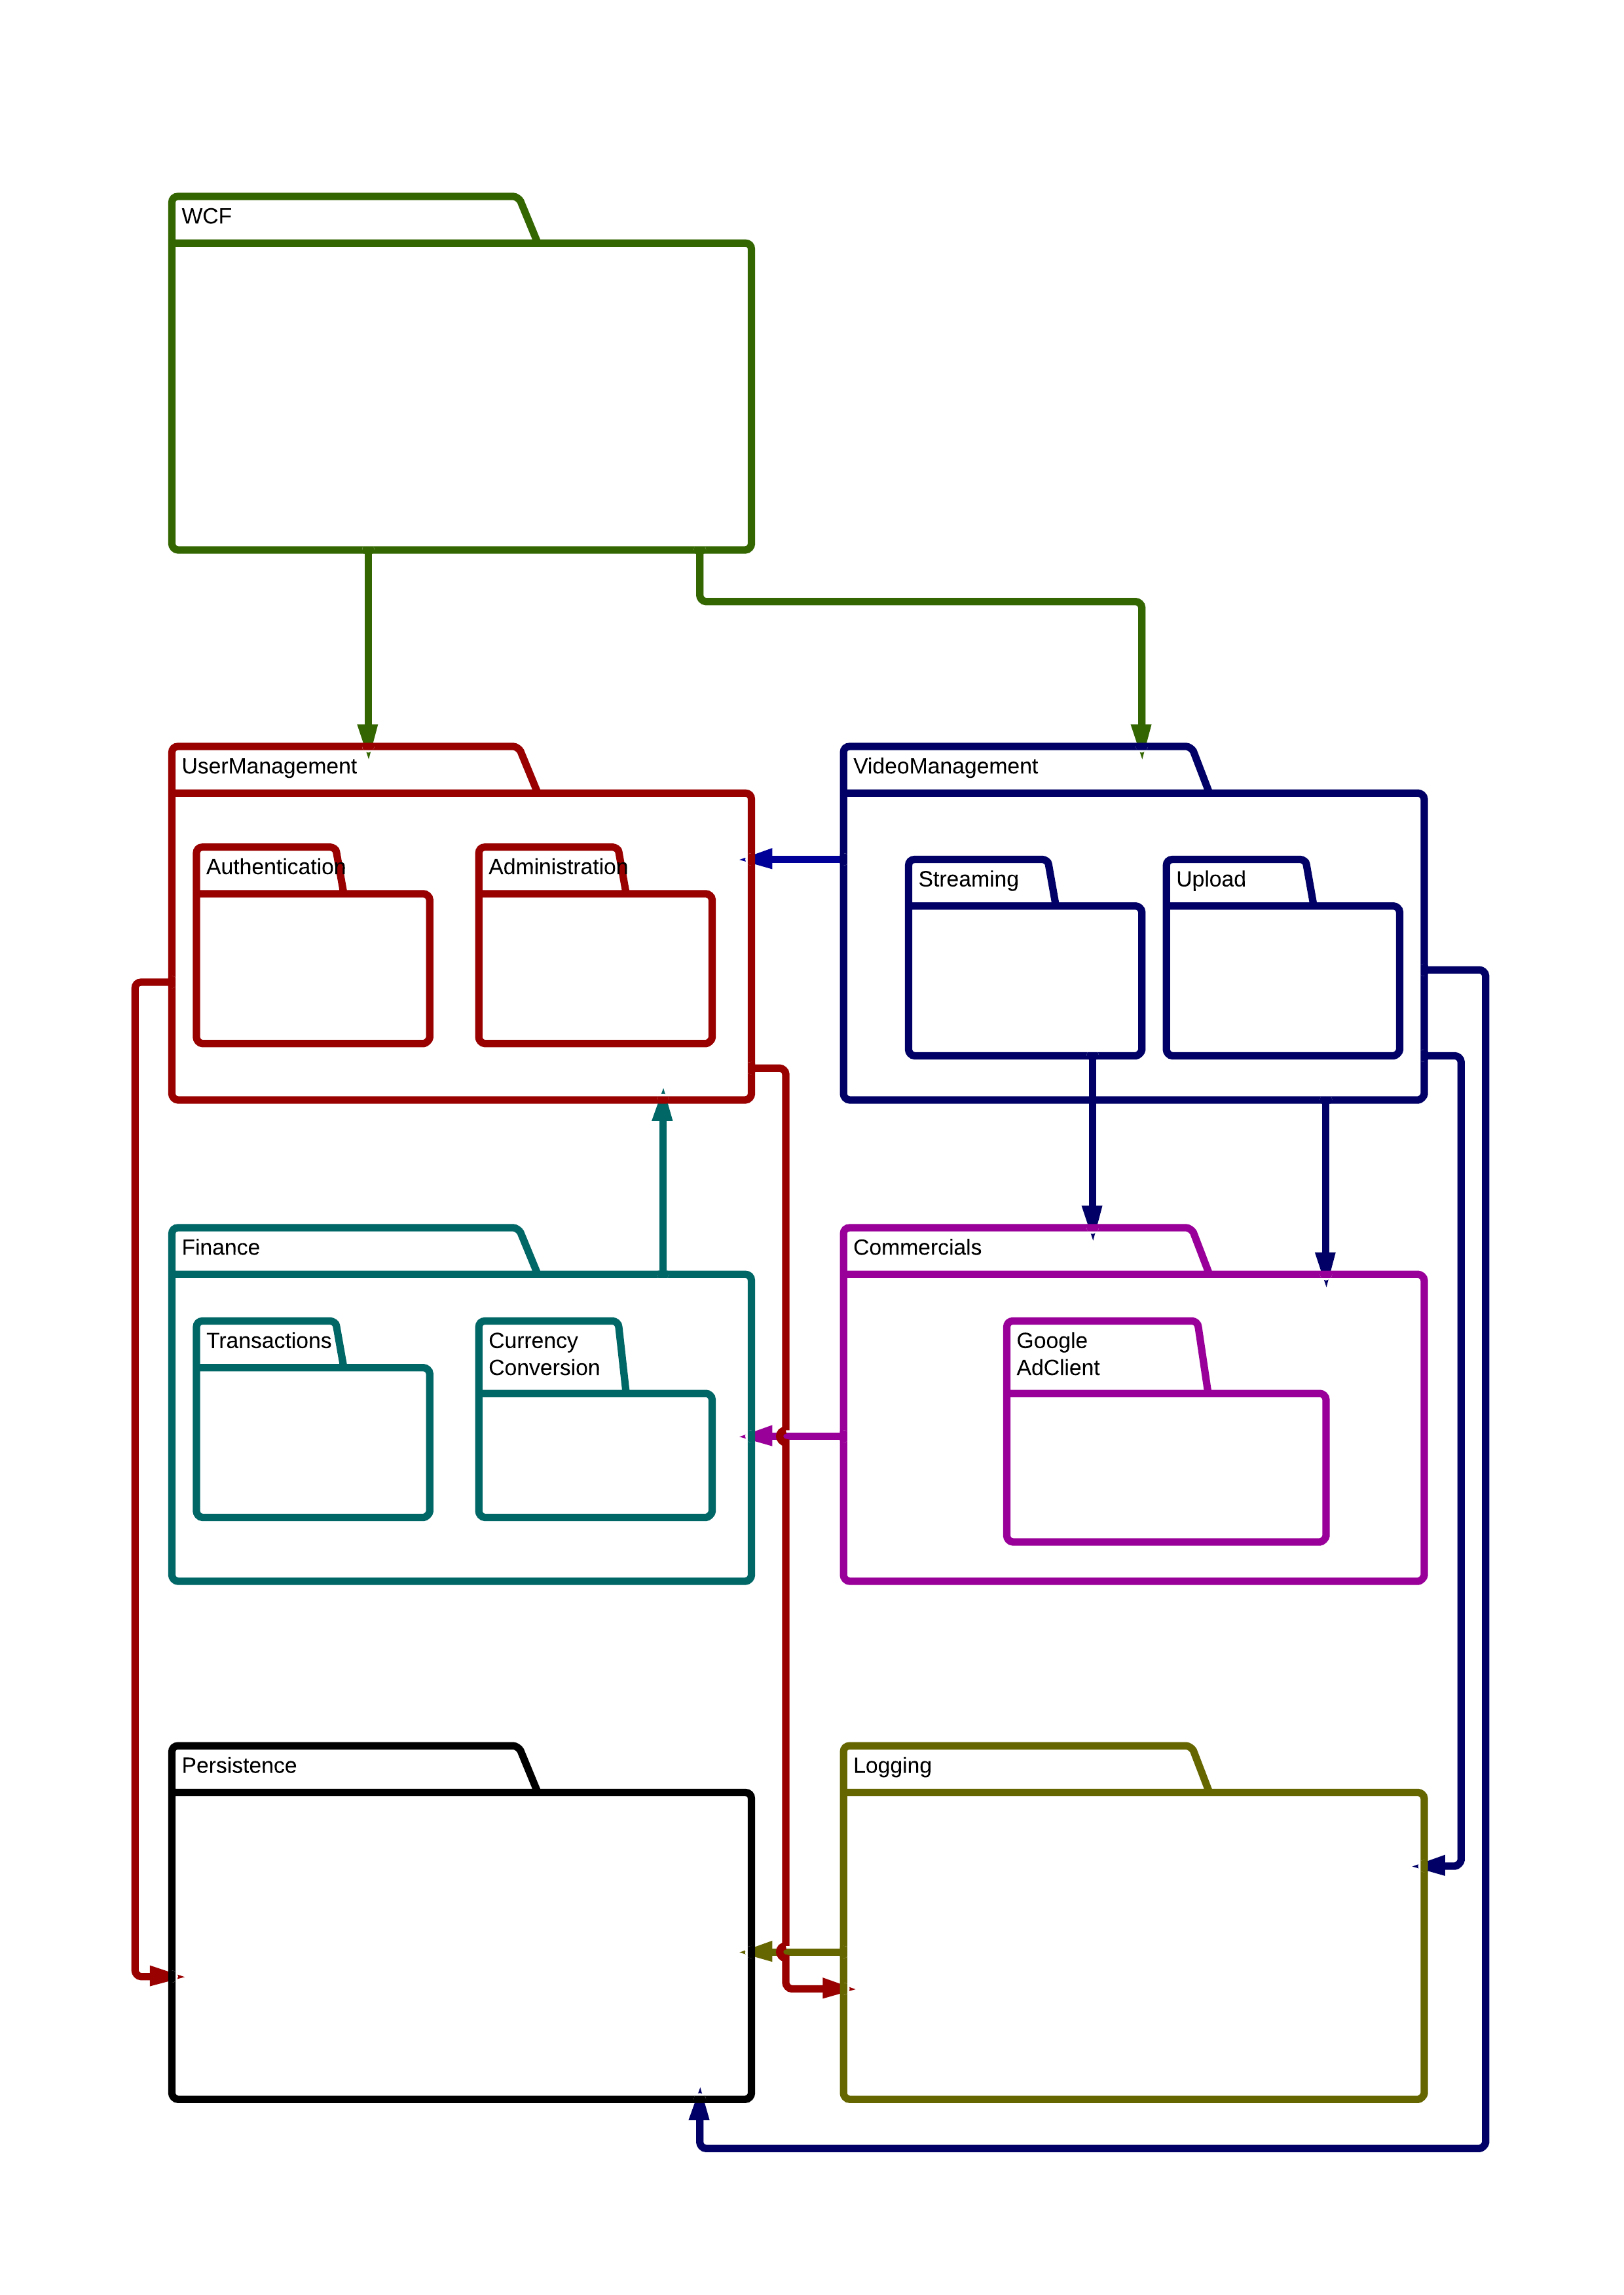
\includegraphics[scale=0.15]{PackageDiagram.png}
\end{center}
\subsection{Technology Considerations}
REST VS SOAP\\
HTML5 vs Silverlight\\
Facebook Login vs WCF login\\
PayPal\\
Ads\\
Preventing unauthorized downloading\\
\section{Project Management Plan}